% Based on the template https://github.com/Noktec/Abertay_Beamer_Template
\documentclass[aspectratio=169, 169]{beamer}
% Use \documentclass{beamer} for narrow template
\usetheme{STR}
\usepackage{caption}
\usepackage{gensymb}
\newcommand\myheading[1]{%
  \par\bigskip
  {\Large\bfseries#1}\par\smallskip}


\title{\linebreak Vue.js}
%\subtitle{Subtitle}
\author{ Anandhakrishnan M\linebreak
S7 CSA \\ Guided By:\\ Mr. Muhammed Ilyas H
}


% Uncomment to use your own affiliation, otherwise, default is used
%\renewcommand{\addresstext}{https://www.overleaf.com/project/5f6199feb3f6070001acd711
%Department of stuff 
%University of school}

\begin{document}
\section{Section 1}

\begin{frame}
    \titlepage
\end{frame}
\begin{frame}{OVERVIEW}
\begin{itemize}
    \item INTRODUCTION
    \item VUE FEATURES
    \item HOW TO INCLUDE VUE.JS IN A PROJECT
    \item HELLO WORLD IN VUE.JS
    \item VUE DIRECTIVES
    \item ADVANTAGES
    \item DISADVANTAGES
    \item LIVE DEMO
    \item CONCLUSION
\end{itemize}
    
\end{frame}


\begin{frame}{INTRODUCTION}
\justifying
\begin{itemize}
\item Vue is a progressive framework for building user interfaces. 
\item The core library is focused on the view layer only, and is easy to pick up and integrate with other libraries or existing projects.  
\item Vue is also perfectly capable of powering complex Single-Page  Applications.
\item Vue is more simple and flexible.
\item Vue allows to make just a specific part of the application
\end{itemize}
\end{frame}
\begin{frame}{EVAN YOU}
    \center
\includegraphics[width=4cm]{evan-you.jpeg}
  \begin{itemize}
      \item  Vue.js was created by Evan You, and is maintained by him and the rest of the active core team members coming from various companies such as Netlify and Netguru.
  \end{itemize}
\end{frame}
\begin{frame}{VUE POPULARITY}
 \center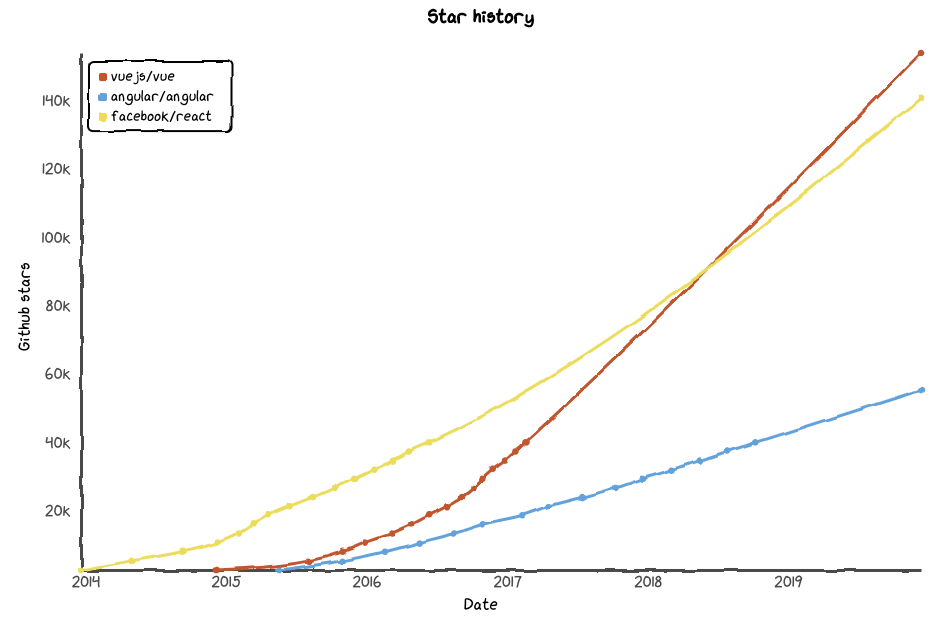
\includegraphics[width=8cm]{vuegithub.png}
\end{frame}
\begin{frame}{VUE POPULARITY CONTD.}
 \center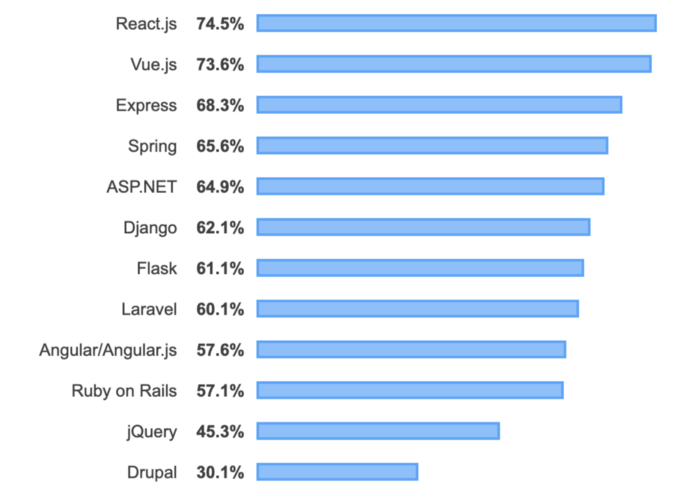
\includegraphics[width=8cm]{vue1.png}
\end{frame}
\begin{frame}{MAJOR VUE USERS}
 \center
\includegraphics[width=8cm]{vue2.png}
\end{frame}
\begin{frame}{VUE FEATURES}
\myheading{Virtual DOM}
\begin{itemize}
    \item Vue.js makes the use of virtual DOM. 
    \item The changes are not made to the DOM, instead a replica of the DOM is created.
    \item  Whenever any changes are to be made, they are made to the Virtual DOM and later it is compared with the original DOM. The final changes are then updated to the real DOM
\end{itemize}
\myheading{Components}
 \begin{itemize}
     \item Components are one of the important features of Vue.js that helps create custom elements, which can be reused in HTML.
 \end{itemize}

\end{frame}
\begin{frame}{VUE FEATURES CONTD.}
 \center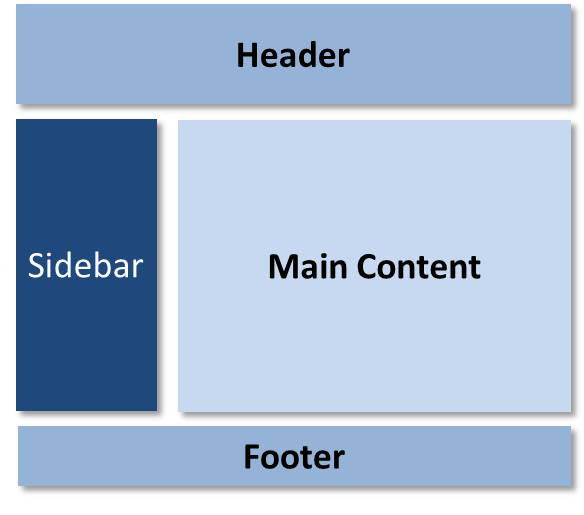
\includegraphics[width=8cm]{Components.jpg}
\end{frame}
\begin{frame}{VUE FEATURES CONTD.}
 \myheading{Event Handling}
  \begin{itemize}
      \item v-on is the attribute added to the DOM elements to listen to the events in Vue.js.
  \end{itemize}
  \myheading{Directives}
  \begin{itemize}
      \item Vue.js has built-in directives such as v-if, v-else, v-show, v-on, v-bind, and v-model, which are used to perform various actions on the frontend
  \end{itemize}
   \myheading{Animation/Transition}
  \begin{itemize}
      \item Vue provides various ways to apply transition to HTML elements when they are added/updated or removed from the DOM
  \end{itemize}
\end{frame}
\begin{frame}{VUE FEATURES CONTD.}
 \myheading{Templates}
 \begin{itemize}
     \item Vue provides HTML-based templates
     \item Vue uses html, js and css separately. 
     \item It is very easy for a beginner to understand and adopt the VueJS style.
 \end{itemize}
    
\end{frame}

\begin{frame}{HOW TO INCLUDE VUE JS IN A PROJECT}
\justifying
\begin{itemize}
   \item Include Vue CDN in link in a script tag
   \center\larege\url{https://cdn.jsdelivr.net/npm/vue@2.6.12}
   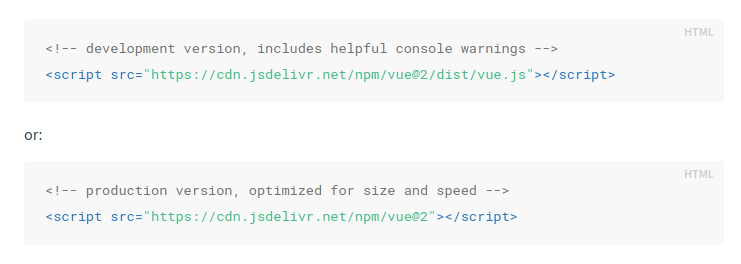
\includegraphics[width=9.5cm]{vueSetup.png}
   \end{itemize}
  
    
\end{frame}

\begin{frame}{HELLO WORLD IN VUE.JS}
    %\centering
    %\Huge{\textbf{Separator Slide}}
\begin{itemize}
\item  Html part
\linebreak

\center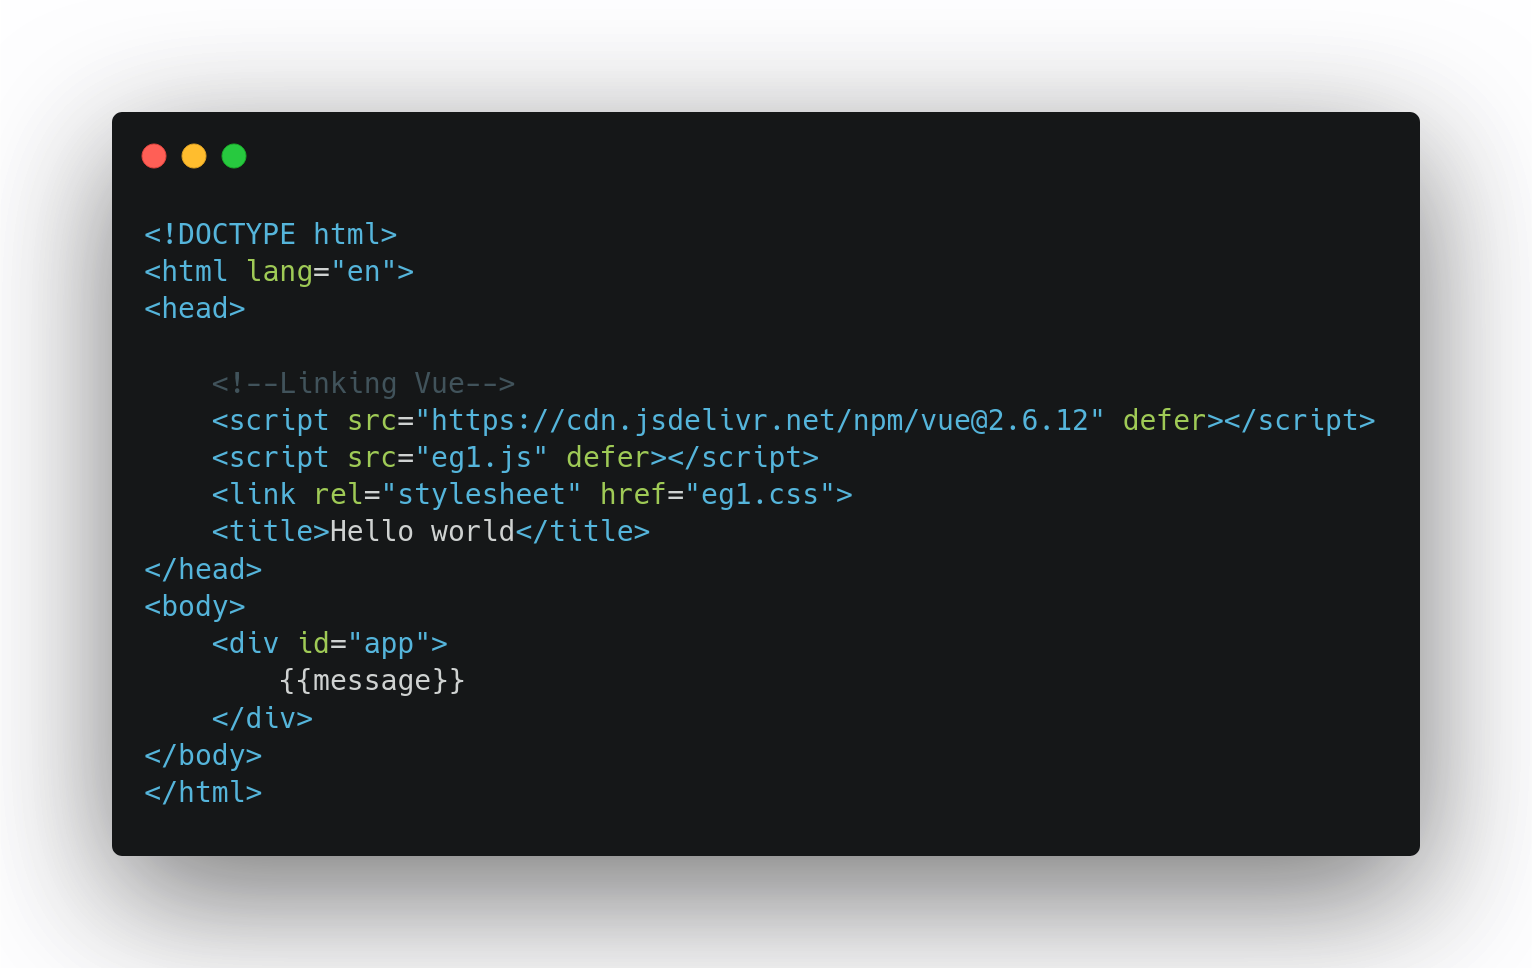
\includegraphics[width=10cm]{vuehelloworld.png}
\end{itemize}
\end{frame}
\begin{frame}{HELLO WORLD IN VUE.JS CONTD.}
    %\centering
    %\Huge{\textbf{Separator Slide}}
\begin{itemize}
\item Js Part
\linebreak

\center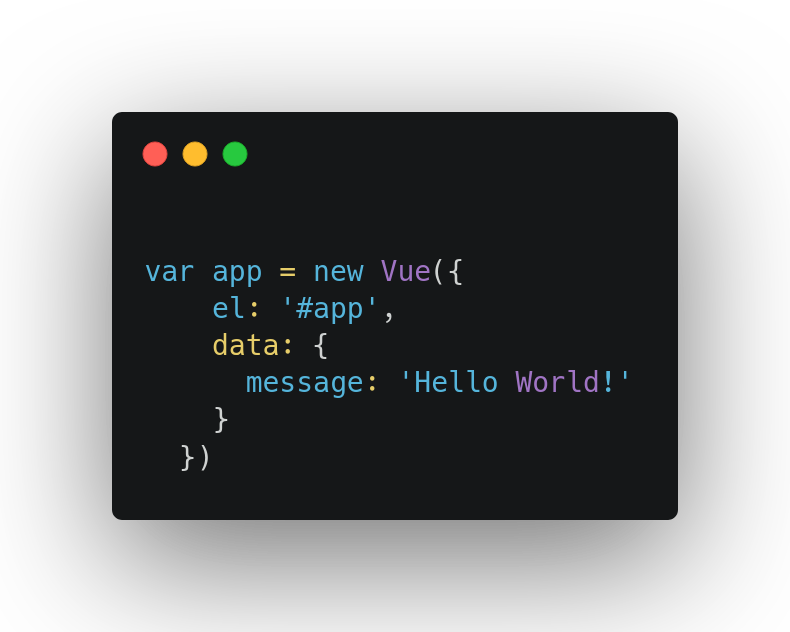
\includegraphics[width=8cm]{helloWorldJs.png}
\end{itemize}
\end{frame}
\begin{frame}{VUE DIRECTIVES}
  \myheading{v-if}
  \begin{itemize}
      \item The directive v-if is used to conditionally render a block. 
      \item The block will only be rendered if the directive’s expression returns a truthy value.
  \end{itemize}
   \myheading{v-for}
  \begin{itemize}
      \item The directive v-for to render a list of items based on an array 
      
  \end{itemize}
  \myheading{v-on}
  \begin{itemize}
      \item  v-on directive is used  to listen DOM events and run some JavaScript when they’re triggered. 
      
  \end{itemize}
\end{frame}
\begin{frame}{VUE DIRECTIVES CONTD.}
    \myheading{v-model}
  \begin{itemize}
      \item The v-model directive is  used to create two-way data bindings on form input, textarea, and select elements. 
      \item It automatically picks the correct way to update the element based on the input type. 
      
  \end{itemize}
\end{frame}
\begin{frame}{ ADVANTAGES }
    \begin{itemize}
        \item Small size
        \item Good documentation 
        \item Easy to understand
        \item Simple integration
    \end{itemize}
\end{frame}
\begin{frame}{ DISADVANTAGES }
    \begin{itemize}
        \item Less Resources
        \item No tech-giants for backing up vue
    \end{itemize}
\end{frame}
\begin{frame}{LIVE DEMO}
    \center
\includegraphics[width=8cm]{livedemo.png}
     \center\larege\url{http://127.0.0.1:5500/index.html}
\end{frame}
\begin{frame}{CONCLUSION}
    \begin{itemize}
        \item Vue is a simple progressive framework for front end development
        \item Vue is easy to learn 
        \item Easy to integrate with an existing project
        \item virtual DOM concepts helps to improve the speed of the application
        \item Concepts of web components helps to reuse the code
    \end{itemize}
\end{frame}

\begin{frame}{REFERENCE}
    \begin{itemize}
        \item [1] https://vuejs.org/v2/guide/index.html
        \item [2] https://www.tutorialspoint.com/vuejs/index.htm
        \item [3] https://en.wikipedia.org/wiki/Vue.js
        \item [4] https://medium.com/@ronak8036/pros-and-cons-of-the-vue-js-framework-8015dcbc05ef
        \item [5] https://github.com/vuejs/vue
        \item [6] https://towardsdatascience.com/what-are-the-pros-and-cons-of-using-vue-js-3689d00d87b0s

    \end{itemize}
\end{frame}
\begin{frame}
\centering \Huge
\emph{Thank You\\for Listening.}
\end{frame}

\end{document}
